%\hypertarget{___gatsby}{}
%\hypertarget{gatsby-focus-wrapper}{}
%\href{https://mukulrathi.com/}{}
%
%MUKUL RATHI
%
%\href{https://mukulrathi.com/about-me}{}
%
%About Me
%
%\href{https://mukulrathi.com/blog}{}
%
%Blog
%
%\hypertarget{creating-the-bolt-compiler-part-9}{%
%\subsection{Creating the Bolt Compiler: Part
%9}\label{creating-the-bolt-compiler-part-9}}

\hypertarget{top-of-page}{%
\chapter{Implementing Concurrency and our Runtime
Library}\label{top-of-page}}

December 28, 2020

%\hypertarget{december-28-2020}{%
%\subsection{December 28, 2020}\label{december-28-2020}}
%
%\hypertarget{min-read}{%
%\subsection{9 min read}\label{min-read}}

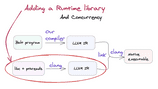
\includegraphics[width=\linewidth]{09_files/runtime-library.png}

%\hypertarget{series-creating-the-bolt-compiler}{%
%\section{Series: Creating the Bolt
%Compiler}\label{series-creating-the-bolt-compiler}}
%
%\begin{itemize}
%\item
%  { Part 1:
%  }\href{https://mukulrathi.com/create-your-own-programming-language/intro-to-compiler/}{How
%  I wrote my own "proper" programming language}
%\item
%  { Part 2:
%  }\href{https://mukulrathi.com/create-your-own-programming-language/compiler-engineering-structure/}{So
%  how do you structure a compiler project?}
%\item
%  { Part 3:
%  }\href{https://mukulrathi.com/create-your-own-programming-language/parsing-ocamllex-menhir/}{Writing
%  a Lexer and Parser using OCamllex and Menhir}
%\item
%  { Part 4:
%  }\href{https://mukulrathi.com/create-your-own-programming-language/intro-to-type-checking/}{An
%  accessible introduction to type theory and implementing a
%  type-checker}
%\item
%  { Part 5:
%  }\href{https://mukulrathi.com/create-your-own-programming-language/data-race-dataflow-analysis/}{A
%  tutorial on liveness and alias dataflow analysis}
%\item
%  { Part 6:
%  }\href{https://mukulrathi.com/create-your-own-programming-language/lower-language-constructs-to-llvm/}{Desugaring
%  - taking our high-level language and simplifying it!}
%\item
%  { Part 7:
%  }\href{https://mukulrathi.com/create-your-own-programming-language/protobuf-ocaml-cpp-tutorial/}{A
%  Protobuf tutorial for OCaml and C++}
%\item
%  { Part 8:
%  }\href{https://mukulrathi.com/create-your-own-programming-language/llvm-ir-cpp-api-tutorial/}{A
%  Complete Guide to LLVM for Programming Language Creators}
%\item
%  \textbf{Part 9: Implementing Concurrency and our Runtime Library}
%\item
%  { Part 10:
%  }\href{https://mukulrathi.com/create-your-own-programming-language/generics-parametric-polymorphism/}{Generics
%  - adding polymorphism to Bolt}
%\item
%  { Part 11:
%  }\href{https://mukulrathi.com/create-your-own-programming-language/inheritance-method-overriding-vtable/}{Adding
%  Inheritance and Method Overriding to Our Language}
%\end{itemize}
%
%\begin{center}\rule{0.5\linewidth}{0.5pt}\end{center}

\hypertarget{the-role-of-a-runtime-library}{%
\section{\texorpdfstring{\protect\hyperlink{the-role-of-a-runtime-library}{}The
Role of a Runtime
Library}{The Role of a Runtime Library}}\label{the-role-of-a-runtime-library}}

Up till now, we've translated constructs in our language Bolt directly
into LLVM IR instructions. The biggest misconception I had with
concurrency was that it worked in the same manner. That there was some
\texttt{spawn} instruction that compilers could emit that would create a
new thread. This isn't the case. LLVM doesn't have a single instruction
to create threads for you. Why not, you ask? What's so special about
threads?

Creating a thread is a complex routine of instructions that are
\textbf{platform-specific}. Threads are managed by the OS kernel, so
creating a thread involves creating system calls following that
platform's conventions.

LLVM draws a line here. There's a limit to how much functionality LLVM
can provide without itself becoming \emph{huge}. Just think of the
variety of platforms out there that it would have to support, from
embedded systems to mobile to the different desktop OSs.

Enter your \textbf{runtime library}. Your language's runtime library
provides the \emph{implementation} for these routines that interact with
the platform / runtime environment. The compiler inserts calls to these
runtime library functions when compiling our Bolt program. Once we have
our compiled LLVM IR, we \textbf{link} in the runtime library function
implementations, so the executable can call these.

You know what the best part is about compiling to LLVM IR? We don't have
to write our own runtime library. C compiles to LLVM IR. Let's just use
C functions to bootstrap our runtime library and \texttt{clang} to link
them in!

So which kinds of functions are present in our runtime library?

\begin{itemize}
\tightlist
\item
  I/O e.g. \texttt{printf}
\item
  Memory management. (Remember in the previous post I mentioned that the
  LLVM didn't provide a heap.) Either implemented manually
  (\texttt{malloc} and \texttt{free}) or through a garbage collection
  algorithm (e.g. \emph{mark-and-sweep}).
\item
  And of course \textbf{threads} via the C \texttt{pthread} API. Pthread
  is short for \href{https://en.wikipedia.org/wiki/POSIX_Threads}{POSIX
  Thread}, a standardised API for these thread system calls.
\end{itemize}

We aren't just limited to the functions provided by C. We can write our
own C functions and link them in using the techniques described in this
post.

We'll look at \texttt{printf}

\hypertarget{recap-llvm-module}{%
\section{\texorpdfstring{\protect\hyperlink{recap-llvm-module}{}Recap:
LLVM Module}{Recap: LLVM Module}}\label{recap-llvm-module}}

Here's a quick sketch of the structure of an LLVM module (from the
\href{https://mukulrathi.com/create-your-own-programming-language/llvm-ir-cpp-api-tutorial/}{previous
post}). As the diagram shows, the part of the module we're interested in
is the \textbf{function declarations}. To use a C library function, we
need to insert its function signature in our module's function
declarations symbol table.

{
\href{https://mukulrathi.com/static/e21edb9623d8fb7bc23f57db23b93cf8/cad61/module.png}{{}
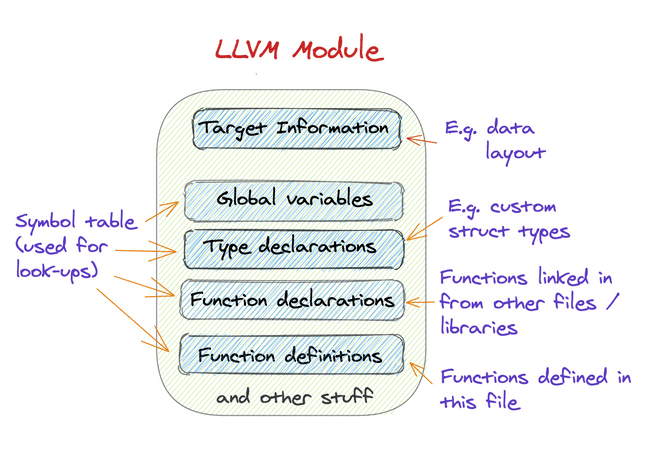
\includegraphics[width=\linewidth]{09_files/module.png}} }

\hypertarget{printf}{%
\section{\texorpdfstring{\protect\hyperlink{printf}{}Printf}{Printf}}\label{printf}}

Let's warm up with \texttt{printf}. The C function type signature is:

%Copy

\begin{lstlisting}[language=C]
int printf ( const char* format, ... );
\end{lstlisting}

To translate this C type signature to an LLVM \texttt{FunctionType}:

\begin{itemize}
\tightlist
\item
  drop the \texttt{const} qualifier
\item
  Convert C types to equivalent LLVM types: \texttt{int} and
  \texttt{char} map to \texttt{i32} and \texttt{i8} respectively
\item
  the \texttt{...} indicates \texttt{printf} is variadic. So the LLVM
  API code is as follows:
\end{itemize}

%{
%\href{https://github.com/mukul-rathi/bolt/blob/master/src/llvm-backend/llvm_ir_codegen/extern_functions_codegen.cc\#L17-L21}{extern\_functions\_codegen.cc}}
%
%Copy

\begin{lstlisting}[language=C++,caption={extern\_functions\_codegen.cc}]
module->getOrInsertFunction(  "printf",  FunctionType::get(    IntegerType::getInt32Ty(*context),    Type::getInt8Ty(*context)->getPointerTo(),    true /* this is variadic func */  ));
\end{lstlisting}

And the corresponding code to call the \texttt{printf} function:

%{
%\href{https://github.com/mukul-rathi/bolt/blob/master/src/llvm-backend/llvm_ir_codegen/expr_codegen.cc\#L412-L424}{expr\_codegen.cc}}
%
%Copy

\begin{lstlisting}[caption={expr\_codegen.cc},language=C++]
Value *IRCodegenVisitor::codegen(const ExprPrintfIR &expr) {
  Function *printf = module->getFunction("printf");
  std::vector<Value *> printfArgs;
  Value *formatStrVal = builder->CreateGlobalStringPtr(expr.formatStr);
  printfArgs.push_back(formatStrVal);
  // add variadic arguments
  for (auto &arg : expr.arguments) {
    printfArgs.push_back(arg->codegen(*this););
  }
  return builder->CreateCall(printf, printfArgs);
};
\end{lstlisting}

\href{https://llvm.org/doxygen/classllvm_1_1IRBuilderBase.html\#abd2f5469db2235e00ac6df61fe766c85}{CreateGlobalStringPtr}
is a useful \texttt{IRBuilder} method that takes in a string and returns
an \texttt{i8*} pointer (so we have a argument of the right type).

\hypertarget{the-bolt-memory-model}{%
\section{\texorpdfstring{\protect\hyperlink{the-bolt-memory-model}{}The
Bolt Memory Model}{The Bolt Memory Model}}\label{the-bolt-memory-model}}

Each thread has \textbf{its own stack}. To share objects between
threads, we'll introduce a \textbf{global heap} of objects. We'll use
the stack to store primitives like ints, bools and to store pointers to
objects on the heap.

{
\href{https://mukulrathi.com/static/f9e2f9b192e5a29e4bca4304ec811151/b4904/hardware-threads.png}{{}
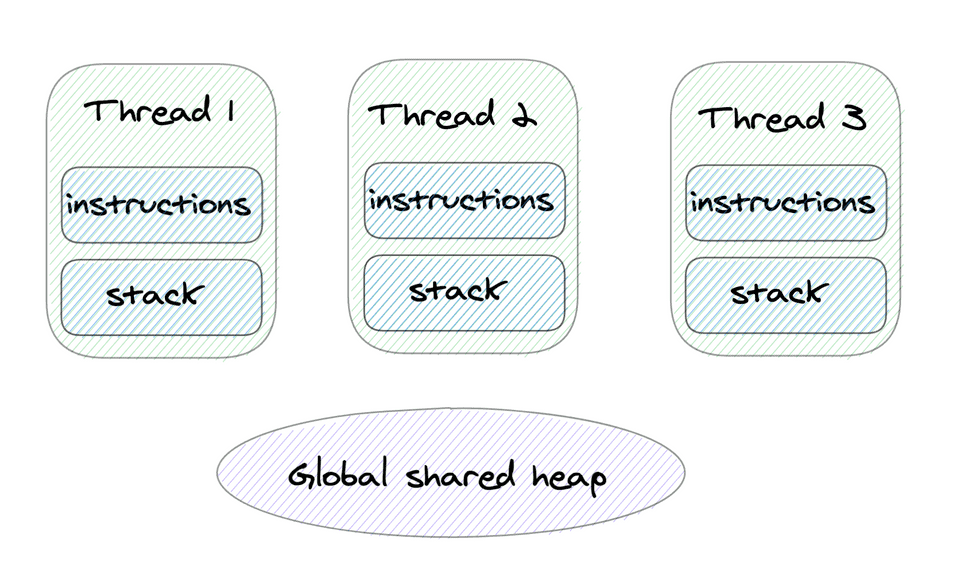
\includegraphics[width=\linewidth]{09_files/hardware-threads.png}} }

{
\href{https://mukulrathi.com/static/ff99489ea7fb99d5a54e6d5a32342340/e53e8/stack-heap.png}{{}
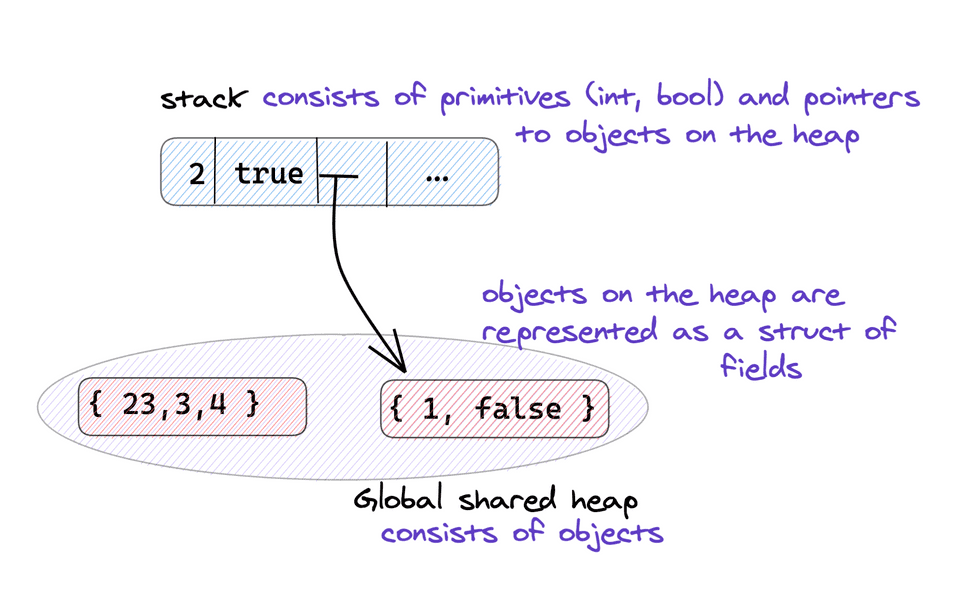
\includegraphics[width=\linewidth]{09_files/stack-heap.png}} }

\hypertarget{malloc}{%
\subsection{\texorpdfstring{\protect\hyperlink{malloc}{}Malloc}{Malloc}}\label{malloc}}

We can use \texttt{malloc} to allocate objects to the heap. (This is
what C++`s \texttt{new} keyword does under the hood!)

The type signature for \texttt{malloc} is as follows:

%Copy

\begin{lstlisting}[language=C]
void *malloc(size_t size);
\end{lstlisting}

Converting this to the equivalent LLVM IR types, \texttt{void\ *} and
\texttt{size\_t} map to \texttt{i8\ *} and \texttt{i64}. The LLVM API
code falls out once you've determined the LLVM types.

%{
%\href{https://github.com/mukul-rathi/bolt/blob/master/src/llvm-backend/llvm_ir_codegen/extern_functions_codegen.cc\#L23-L32}{extern\_functions\_codegen.cc}}
%
%Copy

\begin{lstlisting}[caption={extern\_functions\_codegen.cc},language=C++]
Type *voidPtrTy = Type::getInt8Ty(*context)->getPointerTo();
module->getOrInsertFunction(
  "malloc",  FunctionType::get(
    voidPtrTy,
    IntegerType::getInt64Ty(*context),
    /* has variadic args */ false  ));
\end{lstlisting}

There is just one issue though. When we create a \texttt{struct} on the
heap, \texttt{malloc} requires us to specify the number of bytes we want
to allocate. However the size of that \texttt{struct} is
machine-specific information (it depends on the size of datatype, struct
padding etc.). How do we do this in LLVM IR, which is
machine-independent?

We can compute this through the following \emph{hack}. We know that an
array of structs of type \texttt{Foo} is just a contiguous block of
memory. Pointers to adjacent indices are \texttt{size(Foo)} bytes apart.
Therefore, if we start an array at address \texttt{0x0000} (the special
\texttt{NULL} address) then the first index of the array is at address
\texttt{size(Foo)}.

{
\href{https://mukulrathi.com/static/3ffd7d3a6019e3375f7834e25b4853f8/95fa1/malloc-size.png}{{}
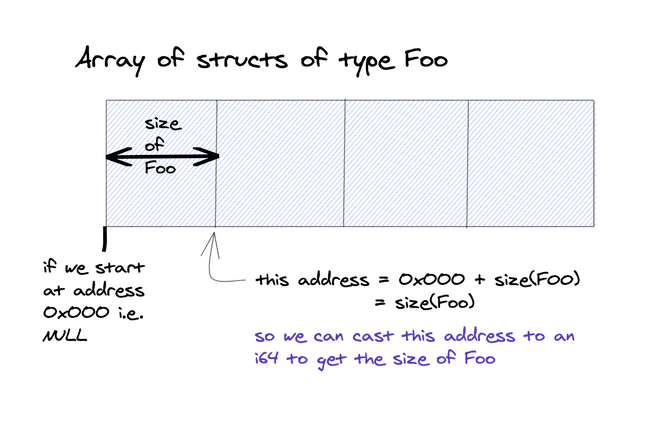
\includegraphics[width=\linewidth]{09_files/malloc-size.png}} }

We can use the \texttt{getelementptr} (GEP) instruction to compute this
array address, and pass in the base pointer of the array as the
\texttt{null} value. You might be thinking, hold on, this array doesn't
exist. Won't this cause a seg fault?

Remember, the role of the GEP instruction is just to calculate pointer
offsets. Not to check if the resultant pointer is valid. Not to actually
access the memory. Just to perform this calculation. No memory access =
no seg fault.

%{
%\href{https://github.com/mukul-rathi/bolt/blob/master/src/llvm-backend/llvm_ir_codegen/expr_codegen.cc\#L74-L83}{expr\_codegen.cc}}
%
%Copy

\begin{lstlisting}[language=C++,caption={expr\_codegen.cc}]
// calculate index of array[1] using GEP instructionValue *objDummyPtr = builder->CreateConstGEP1_64(    Constant::getNullValue(objType->getPointerTo()), 1, "objsize");// cast to i64 for mallocValue *objSize =    builder->CreatePointerCast(objDummyPtr,Type::getInt64Ty(*context));
\end{lstlisting}

We pass \texttt{objSize} to \texttt{malloc}. \texttt{malloc} returns a
\texttt{void\ *} pointer, however since we will later want to access the
struct's fields, we need to cast the type to \texttt{objType*}.
Remember, LLVM needs explicit types!

%{
%\href{https://github.com/mukul-rathi/bolt/blob/master/src/llvm-backend/llvm_ir_codegen/expr_codegen.cc\#L74-L83}{expr\_codegen.cc}}
%
%Copy

\begin{lstlisting}[language=C++,caption={expr\_codegen.cc}]
// allocate the object on the heap
Value *objVoidPtr =
    builder->CreateCall(module->getFunction("malloc"), objSize);
// cast (void *)  to  (objType *)
Value *obj =    builder->CreatePointerCast(objVoidPtr, objType->getPointerTo());
\end{lstlisting}

\hypertarget{bonus-garbage-collection}{%
\subsection{\texorpdfstring{\protect\hyperlink{bonus-garbage-collection}{}Bonus:
Garbage
Collection}{Bonus: Garbage Collection}}\label{bonus-garbage-collection}}

Swap out \texttt{malloc} for \texttt{GC\ malloc}. If we use
\href{https://linux.die.net/man/3/gc}{GC\_malloc}, we get garbage
collection for free! How cool is that?! We don't need to \texttt{free()}
our object.

If you want to implement your own garbage collector,
\href{https://llvm.org/docs/GarbageCollection.html}{check this LLVM page
out}.

\hypertarget{implementing-hardware-threads-with-pthreads}{%
\section{\texorpdfstring{\protect\hyperlink{implementing-hardware-threads-with-pthreads}{}Implementing
Hardware Threads with
Pthreads}{Implementing Hardware Threads with Pthreads}}\label{implementing-hardware-threads-with-pthreads}}

So far we've looked at \texttt{printf} and \texttt{malloc}. We've found
that the biggest hurdle to declaring their function signatures is
translating C types to LLVM IR types. Once you have the LLVM IR types,
everything falls out. With the \texttt{pthread} API the process is the
same, only the translation from C types to LLVM IR types is a little
more involved.

\hypertarget{understanding-the-pthread-api}{%
\subsection{\texorpdfstring{\protect\hyperlink{understanding-the-pthread-api}{}Understanding
the Pthread
API}{Understanding the Pthread API}}\label{understanding-the-pthread-api}}

The two functions we'd like to use to create and join threads are
\href{https://man7.org/linux/man-pages/man3/pthread_create.3.html}{pthread\_create}
and
\href{https://man7.org/linux/man-pages/man3/pthread_join.3.html}{pthread\_join}.
The linked Linux manual pages give a full description of the functions,
but they are a bit dense.

Let's unpack the relevant information, starting with the function
signatures:

%Copy

\begin{lstlisting}[language=C]
int pthread_create(pthread_t *thread, const pthread_attr_t *attr,
                          void *(*start_routine) (void *), void *arg);
int pthread_join(pthread_t thread, void **retval);
\end{lstlisting}

Both \texttt{pthread\_create} and \texttt{pthread\_join} are idiomatic C
functions in that:

\begin{itemize}
\tightlist
\item
  they return an \texttt{int}, where the value \texttt{0} = success and
  other values = error codes.
\item
  to return additional values e.g a \texttt{val} of type \texttt{Foo},
  we pass in a \emph{pointer} \texttt{p} of type \texttt{Foo*} as an
  argument. The function will update the pointer's value to that
  returned value (\texttt{*p=val}). We can then access the returned
  value by dereferencing the pointer (\texttt{*p}).
  \href{https://www.ibm.com/support/knowledgecenter/SSLTBW_2.4.0/com.ibm.zos.v2r4.cbclx01/pass_by_pointer.htm}{See
  this tutorial} if you're not familiar with this
  \emph{``pass-by-pointer''} pattern.
\end{itemize}

If you're not familiar with C pointer syntax,
\texttt{void\ *(*start\_routine)\ (void\ *)} is quite a mouthful. This
says \texttt{start\_routine} is a pointer to a function that takes in a
\texttt{void\ *} argument and returns a \texttt{void\ *} value.
\texttt{void\ *} is the generic type representing \emph{any} pointer
(it's super flexible - we can cast it to any type we'd like e.g.
\texttt{int\ *} or \texttt{Foo\ *}).

\texttt{pthread\_create} creates a thread, which will asynchronously
execute the function pointed to by \texttt{start\_routine} with the
\texttt{arg} argument. The opaque \texttt{pthread\_t} type represents a
handle to a thread object (can think of it like a thread id ). We pass a
\texttt{pthread\_t\ *} pointer, and \texttt{pthread\_create} will assign
the \texttt{pthread\_t} handle corresponding to the created thread to
this object. The opaque \texttt{pthread\_attr\_t} type represents any
attributes we want the thread to have. The \texttt{pthread\_attr\_t\ *}
parameter lets us specify the attributes we want the created thread to
have. Passing \texttt{NULL} will initialise the thread with default
attributes, which is good enough for us.

We pass the \texttt{pthread\_t} handle to \texttt{pthread\_join} to tell
it which thread we are joining (waiting on to finish).
\texttt{pthread\_join} updates the \texttt{void\ **} pointer parameter
with the \texttt{void\ *} return value of \texttt{start\_routine(arg)}
executing on that thread. We can pass \texttt{NULL} if we don't want
this return value.

Here's an
\href{https://timmurphy.org/2010/05/04/pthreads-in-c-a-minimal-working-example/}{excellent
minimal C example} that demonstrates the use of Pthreads.

\hypertarget{translating-pthread-types-into-llvm-ir}{%
\subsection{\texorpdfstring{\protect\hyperlink{translating-pthread-types-into-llvm-ir}{}Translating
Pthread types into LLVM
IR}{Translating Pthread types into LLVM IR}}\label{translating-pthread-types-into-llvm-ir}}

We've seen \texttt{int} and \texttt{void\ *} before: they may to
\texttt{i32} and \texttt{i8*}. \texttt{void\ **} follows as
\texttt{i8*}. We're in a bit of a pickle with \texttt{pthread\_t} and
\texttt{pthread\_attr\_t} as their type definitions are opaque.

Aw shucks, we're stuck. The solution (as with most cases when you're
stuck with LLVM IR) is to \textbf{experiment in C and look at the
compiled LLVM IR output}.

We can compile that
\href{https://timmurphy.org/2010/05/04/pthreads-in-c-a-minimal-working-example/}{excellent
minimal C example} to LLVM IR using \texttt{clang}. The command to do
this for a \texttt{foo.c} file is:

%Copy

\begin{verbatim}
clang -S -emit-llvm -O1 foo.c
\end{verbatim}

The Clang LLVM IR output is quite messy. The best way to read the output
is to find the lines of LLVM IR that correspond to the interesting lines
of code in the C program, and ignore the noise around them. More
information about experimenting with C and C++ to understand LLVM IR in
this
\href{https://www.reddit.com/r/programming/comments/kjjijf/a_complete_guide_to_llvm_for_programming_language/gh2dnnj?utm_source=share\&utm_medium=web2x\&context=3}{excellent
Reddit comment}.

For us, the interesting lines are those that allocate a
\texttt{pthread\_t} stack variable, and the \texttt{pthread\_create} and
\texttt{pthread\_join} calls:

%Copy
\begin{lstlisting}[language=C,caption={C}]
// C
pthread_t inc_x_thread;
...
pthread_create(&inc_x_thread, NULL, inc_x, &x)
...
pthread_join(inc_x_thread, NULL)
\end{lstlisting}

\begin{lstlisting}[language=llvm,caption={LLVM IR}]
%4 = alloca %struct._opaque_pthread_t*, align 8...
%9 = call i32 @pthread_create(%struct._opaque_pthread_t** %4, %struct._opaque_pthread_attr_t* null, i8* (i8*)* @inc_x, i8* %8)...
%23 = call i32 @pthread_join(%struct._opaque_pthread_t* %22, i8** null)
\end{lstlisting}


If we match up our type definitions for the functions:

%Copy

\begin{lstlisting}[language=llvm]
// C type -> LLVM IR 
typepthread_t = %struct._opaque_pthread_t*pthread_attr_t = %struct._opaque_pthread_attr_t
\end{lstlisting}

Great, we've determined \texttt{pthread\_t} is a pointer to a struct of
type \texttt{\%struct.\_opaque\_pthread\_t}. What's the type of this
struct? Let's look at the type definitions defined earlier in the file:

%Copy

\begin{lstlisting}[language=llvm]
struct.__sFILE = type { i8*, i32, i32, i16, i16, %struct.__sbuf, i32, i8*, i32(i8*)*, i32 (i8*, i8*, i32)*, i64 (i8*, i64, i32)*, i32 (i8*, i8*, i32)*, %struct.__sbuf, %struct.__sFILEX*, i32, [3 x i8], [1 x i8], %struct.__sbuf, i32, i64 }%struct.__sFILEX = type opaque%struct.__sbuf = type { i8*, i32 }%struct._opaque_pthread_t = type { i64, %struct.__darwin_pthread_handler_rec*, [8176 x i8] }%struct.__darwin_pthread_handler_rec = type { void (i8*)*, i8*, %struct.__darwin_pthread_handler_rec* }%struct._opaque_pthread_attr_t = type { i64, [56 x i8] }
\end{lstlisting}

Yikes, this is a mess. Here's the thing. We don't have to declare the
internals of the \texttt{struct} because we \textbf{aren't using them}
in our program. So just as \texttt{\%struct.\_\_sFILEX} was defined as
an opaque struct above, we can define our own opaque structs. The
\texttt{pthread} library's files will specify the bodies of the struct
types as it actually manipulates their internals.

%Copy

\begin{lstlisting}[language=C++]
Type *pthread_t = StructType::create(*context, "struct_pthread_t") ->getPointerTo();
Type *pthread_attr_t = StructType::create(*context,"struct_pthread_attr_t")
\end{lstlisting}

The eagle-eyed amongst you might notice these struct names don't match
the names in the file e.g. \texttt{struct\_pthread\_t} vs
\texttt{struct.\_opaque\_pthread\_t}. What gives?

LLVM's types are resolved \textbf{structurally} not by name. So even if
our program has two separate structs \texttt{Foo} and \texttt{Bar}, if
the types of their fields are the same, LLVM will treat them the same.
The name doesn't matter - we can use one in place of the other without
any errors:

%Copy

\begin{lstlisting}[language=llvm]
// Foo == Bar
%Foo = type {i32, i1}
%Bar = type {i32, i1}
\end{lstlisting}

It turns out we can exploit the structural nature of LLVM's type system
to simplify our types further.

See \texttt{pthread\_attr\_t} is only used in one place:
\texttt{pthread\_create}, and there we pass \texttt{NULL} as the
\texttt{pthread\_attr\_t\ *} argument. \texttt{NULL} is the same value
regardless of type, so rather than defining the type
\texttt{pthread\_attr\_t\ *}, we can use \texttt{void\ *} to represent a
generic \texttt{NULL} pointer.

Let's look at \texttt{pthread\_t} next. We know that \texttt{pthread\_t}
is a \textbf{pointer} to some opaque struct, but we never access that
struct anywhere in our program. In fact, the only place
\texttt{pthread\_t}'s type matters is when we're allocating memory on
the stack for it - we need to know the type to know how many bytes to
allocate.

%{
%\href{https://github.com/mukul-rathi/bolt/blob/master/src/llvm-backend/llvm_ir_codegen/expr_codegen.cc\#L401}{expr\_codegen.cc}}
%
%Copy

\begin{lstlisting}[caption={expr\_codegen.cc},language=c++]
Type *pthreadTy = codegenPthreadTy();Value *pthreadPtr =  builder->CreateAlloca(pthreadTy, nullptr, "pthread");
\end{lstlisting}

Here's the thing: \emph{all} pointers have the same size, regardless of
type, as they all store memory addresses. So we can use a generic
pointer type \texttt{void\ *} for \texttt{pthread\_t} too.

%{
%\href{https://github.com/mukul-rathi/bolt/blob/master/src/llvm-backend/llvm_ir_codegen/extern_functions_codegen.cc\#L23-L32}{extern\_functions\_codegen.cc}}
%
%Copy

\begin{lstlisting}[language=C++,caption={extern\_functions\_codegen.cc}]
Type *IRCodegenVisitor::codegenPthreadTy() {   return Type::getInt8Ty(*context)->getPointerTo();}
\end{lstlisting}

The LLVM API code to declare the \texttt{pthread\_create} and
\texttt{pthread\_join} functions is therefore as follows:

%{
%\href{https://github.com/mukul-rathi/bolt/blob/master/src/llvm-backend/llvm_ir_codegen/extern_functions_codegen.cc\#L36-L62}{extern\_functions\_codegen.cc}}
%
%Copy

\begin{lstlisting}[language=C++,caption={extern\_functions\_codegen.cc}]
Type *voidPtrTy = Type::getInt8Ty(*context)->getPointerTo();
Type *pthreadTy = codegenPthreadTy();
Type *pthreadPtrTy = pthreadTy->getPointerTo();
// (void *) fn (void * arg)
FunctionType *funVoidPtrVoidPtrTy = FunctionType::get(  voidPtrTy, ArrayRef<Type *>({voidPtrTy}),  /* has variadic args */ false);
// int pthread_create(pthread_t * thread, const pthread_attr_t * attr,
//                  void * (*start_routine)(void *), void * arg)
// we use a void * in place of pthread_attr_t *
FunctionType *pthreadCreateTy = FunctionType::get(  Type::getInt32Ty(*context),  ArrayRef<Type *>({pthreadPtrTy, voidPtrTy,                (funVoidPtrVoidPtrTy)->getPointerTo(),                voidPtrTy}),  /* has variadic args */ false);
module->getOrInsertFunction("pthread_create", pthreadCreateTy);
// int pthread_join(pthread_t thread, void **value_ptr)
FunctionType *pthreadJoinTy = FunctionType::get(  Type::getInt32Ty(*context),  ArrayRef<Type *>({pthreadTy, voidPtrTy->getPointerTo()}),  /* has variadic args */ false);
module->getOrInsertFunction("pthread_join", pthreadJoinTy);
\end{lstlisting}

\hypertarget{linking-in-the-runtime-library}{%
\section{\texorpdfstring{\protect\hyperlink{linking-in-the-runtime-library}{}Linking
in the Runtime
Library}{Linking in the Runtime Library}}\label{linking-in-the-runtime-library}}

We can use \texttt{clang} to link in the libraries when we compile our
\texttt{foo.ll} file to a \texttt{./foo} executable.

We link in \texttt{pthread} with the \texttt{-pthread} flag.

To link \texttt{GC\_malloc} we need to do two things:

\begin{itemize}
\tightlist
\item
  Include its header files (here they're in the folder
  \texttt{/usr/local/include/gc/}). We use the \texttt{-I} flag to add
  its folder.
\item
  Add the static library \texttt{.a} file:
  \texttt{/usr/local/lib/libgc.a} to the list of files being compiled.
\end{itemize}

{
\href{https://github.com/mukul-rathi/bolt/blob/master/scripts/compile_program.sh}{compile\_program.sh}}

Copy

\begin{verbatim}
clang -O3 -pthread -I/usr/local/include/gc/ foo.ll  /usr/local/lib/libgc.a  -o foo
\end{verbatim}

\hypertarget{generic-approach-to-bootstrapping-with-c-functions}{%
\section{\texorpdfstring{\protect\hyperlink{generic-approach-to-bootstrapping-with-c-functions}{}Generic
Approach to Bootstrapping with C
functions}{Generic Approach to Bootstrapping with C functions}}\label{generic-approach-to-bootstrapping-with-c-functions}}

We've seen 3 examples of C functions used when bootstrapping our runtime
library: \texttt{printf}, \texttt{malloc} and the \texttt{pthread} API.
The generic approach (can skip steps 2 - 4 if you already understand the
function)

\begin{enumerate}
\tightlist
\item
  Get the C function type signature
\item
  Write a minimal example in C
\item
  Compile the C example to LLVM IR and match up the key lines of your
  example with the corresponding lines of IR e.g. function calls
\item
  Simplify any opaque types into more generic types: only define as much
  type info as you need! E.g. if you don't need to know it's a
  \texttt{struct\ *} pointer (because you're not loading it or
  performing GEP instructions), use a \texttt{void\ *}.
\item
  Translate the C types into LLVM IR types
\item
  Declare the function prototype in your module
\item
  Call the function in LLVM IR wherever you need it!
\item
  Link the function in when compiling the executable
\end{enumerate}

\hypertarget{implementing-concurrency-in-bolt}{%
\section{\texorpdfstring{\protect\hyperlink{implementing-concurrency-in-bolt}{}Implementing
Concurrency in
Bolt}{Implementing Concurrency in Bolt}}\label{implementing-concurrency-in-bolt}}

\hypertarget{the-finish-async-construct}{%
\subsection{\texorpdfstring{\protect\hyperlink{the-finish-async-construct}{}The
Finish-Async
Construct}{The Finish-Async Construct}}\label{the-finish-async-construct}}

Bolt uses the \texttt{finish-async} construct for concurrency. The
\texttt{async} keyword spawns (creates) a thread and sets it to execute
the expressions in that \texttt{async} block. The \texttt{finish} block
scopes the lifetime of any threads spawned inside it using the
\texttt{async} keyword - so all spawned threads must \textbf{join} at
the end of the block. This way we've clearly defined the lifetime of our
threads to be that of the \texttt{finish} block.



%Copy

\begin{lstlisting}[caption={{example\_concurrent\_program.bolt}}]
before();
finish{
  async{
    f();
  }
  async{
    g();
    h();
  }
  during();
}
after();
\end{lstlisting}

Illustrating the execution graphically:

\begin{figure}
\centering
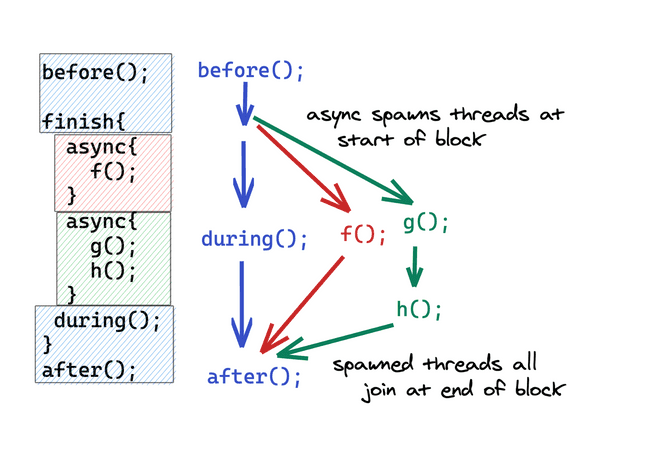
\includegraphics[width=\linewidth]{09_files/finish-async.png}
\caption{A Bolt concurrent program illustrated - each colour represents
a different thread.}
\end{figure}

\hypertarget{creating-our-threads}{%
\subsection{\texorpdfstring{\protect\hyperlink{creating-our-threads}{}Creating
our Threads}{Creating our Threads}}\label{creating-our-threads}}

\hypertarget{compute-free-variables}{%
\paragraph{\texorpdfstring{\protect\hyperlink{compute-free-variables}{}Compute
Free Variables}{Compute Free Variables}}\label{compute-free-variables}}

When inside our \texttt{async} block, we can access any \textbf{objects}
in scope at the start of the \texttt{finish} block (before the
\texttt{async} thread was spawned). For example:

{example\_concurrent\_program.bolt}

Copy

\begin{verbatim}
let a = new Foo();
let b = new Bar();
let y = true;
let z = 2;
finish{
  async{
    // This thread accesses a, b
    let w = 1;
    f(a, b, w);
  }
  ...}
\end{verbatim}

However, there's an issue. In Bolt's memory model, each thread has its
own stack. The \texttt{let\ a\ =\ ...} definition occurs on the main
thread, so the pointer to \texttt{a}'s object is stored on the main
thread's stack. Likewise for \texttt{b}. When we spawn the second thread
using \texttt{async}, this new thread has its own stack, which is empty
(and so doesn't contain \texttt{a} or \texttt{b}).

The first step is to compute the free variables that need to be copied
across to the new stack. Here's a
\href{https://github.com/mukul-rathi/bolt/blob/master/src/frontend/desugaring/desugar_expr.ml\#L140-L141}{link
to the code} if you're interested; we'll skip the details as it's quite
mechanical.
\href{https://mukulrathi.com/create-your-own-programming-language/lower-language-constructs-to-llvm/}{Link
to the previous post on desugaring} if you want to look back at the
desugaring stage.

%Copy

\begin{verbatim}
async{
  //  a, b are free variables
    let w = 1;
    f(a, b, w);
  }
\end{verbatim}

\hypertarget{converting-the-async-block-into-a-function-call}{%
\paragraph{\texorpdfstring{\protect\hyperlink{converting-the-async-block-into-a-function-call}{}Converting
the Async Block into a Function
Call}{Converting the Async Block into a Function Call}}\label{converting-the-async-block-into-a-function-call}}

Now we need to somehow convert this expression into a function that
\texttt{pthread\_create} can run.

%Copy

\begin{verbatim}
async{
    let w = 1;
    f(a, b, w);  }
//  need to convert this to a function
void *asyncFun(void *arg){
  let w = 1;
  f(a, b, w);
  return null;
 // we return null but 
 // you could return the last value instead
}
\end{verbatim}

Since we need all the variables in the function body to be defined, we
need to pass the free variables as arguments to the function:

%Copy

\begin{verbatim}
function void *asyncFun(Foo a, Bar b){
  let w = 1;
  f(a, b, w);
}
let a = new Foo();
let b = new Bar();
let y = true;
let z = 2;
finish{  asyncFun(a, b);  ...}
\end{verbatim}

However, this doesn't match the argument type we're looking for:
\texttt{asyncFun} can only take a \emph{single} \texttt{void*} argument.

The solution: create a \emph{single struct} that contains all of the
values. We can cast the \texttt{struct\ *} to and from a
\texttt{void\ *} pointer to match types.

Copy

\begin{verbatim}
ArgStructType *argStruct = {a, b};// we can cast ArgStructType * to void *asyncFun(argStruct);
\end{verbatim}

Great, now we have the \texttt{void\ *asyncFun(void\ *argStruct)}
function type, as \texttt{pthread\_create} requires.

We need to unpack this inside the function:

%Copy

\begin{verbatim}
function void *asyncFun(void * arg){
  // cast pointer
  ArgStructType *argStruct = (ArgStructType *) arg;
  // unpack variables
  let a = argStruct.a;
  let b = argStruct.b;
  // execute body of function
  let w = 1;
  f(a, b, w);
}
\end{verbatim}

\hypertarget{creating-pthreads}{%
\paragraph{\texorpdfstring{\protect\hyperlink{creating-pthreads}{}Creating
Pthreads}{Creating Pthreads}}\label{creating-pthreads}}

Finally, having defined our arg and our async function, we can invoke
\texttt{pthread\_create}.

The high-level structure of this is as follows:

%{
%\href{https://github.com/mukul-rathi/bolt/blob/master/src/llvm-backend/llvm_ir_codegen/pthread_codegen.cc\#L38-L60}{pthread\_codegen.cc}}
%
%Copy

\begin{lstlisting}[caption={pthread\_codegen.cc},language=C++]
// create async function and argument
  StructType *argStructTy = codegenAsyncFunArgStructType(freeVarList);
  Value *argStruct = codegenAsyncFunArgStruct(asyncExpr, argStructTy);
  Function *asyncFun = codegenAsyncFunction(asyncExpr, argStructTy);
  ...
  // spawn thread
  Function *pthread_create =
      module->getFunction("pthread_create");
  Value *voidPtrNull = Constant::getNullValue(
      Type::getInt8Ty(*context)->getPointerTo());
  Value *args[4] = {
      pthread,
      voidPtrNull,
      asyncFun,
      builder->CreatePointerCast(argStruct, voidPtrTy),  };
  builder->CreateCall(pthread_create, args);
\end{lstlisting}

\texttt{codegenAsyncFunArgStructType}, \texttt{codegenAsyncFunArgStruct}
and \texttt{codegenAsyncFunction} just implement the steps we've
outlined in prose.

\hypertarget{joining-pthreads}{%
\subsection{\texorpdfstring{\protect\hyperlink{joining-pthreads}{}Joining
Pthreads}{Joining Pthreads}}\label{joining-pthreads}}

We join each of the \texttt{pthread\_t} handles for each of the
\texttt{async} expressions' threads.\\
As we mentioned earlier, we aren't returning anything from the
\texttt{asyncFun}, so we can pass in \texttt{NULL} as the second
argument:

%{
%\href{https://github.com/mukul-rathi/bolt/blob/master/src/llvm-backend/llvm_ir_codegen/pthread_codegen.cc\#L14-L25}{pthread\_codegen.cc}}
%
%Copy

\begin{lstlisting}[caption={pthread\_codegen.cc},language=C++]
void IRCodegenVisitor::codegenJoinPThreads(
    const std::vector<Value *> pthreadPtrs) {
  Function *pthread_join =
      module->getFunction("pthread_join");
  Type *voidPtrPtrTy =
      Type::getInt8Ty(*context)->getPointerTo()->getPointerTo();
  for (auto &pthreadPtr : pthreadPtrs) {
    Value *pthread = builder->CreateLoad(pthreadPtr);
    builder->CreateCall(pthread_join,
                        {pthread, Constant::getNullValue(voidPtrPtrTy)});  
  }
\end{lstlisting}

\hypertarget{implementing-finish-async-in-llvm-ir}{%
\subsection{\texorpdfstring{\protect\hyperlink{implementing-finish-async-in-llvm-ir}{}Implementing
Finish-Async in LLVM
IR}{Implementing Finish-Async in LLVM IR}}\label{implementing-finish-async-in-llvm-ir}}

Now we've talked about how we create threads and how we join threads, we
can give the overall code generation for the \texttt{finish-async}
concurrency construct:

%{
%\href{https://github.com/mukul-rathi/bolt/blob/master/src/llvm-backend/llvm_ir_codegen/expr_codegen.cc\#L388-L408}{expr\_codegen.cc}}
%
%Copy

\begin{lstlisting}[caption={expr\_codegen.cc},language=C++]
Value *IRCodegenVisitor::codegen(
    const ExprFinishAsyncIR &finishAsyncExpr) {
  std::vector<Value *> pthreadPtrs;
  // spawn each of the pthreads
  for (auto &asyncExpr : finishAsyncExpr.asyncExprs) {
    Type *pthreadTy = codegenPthreadTy();
    Value *pthreadPtr =
        builder->CreateAlloca(pthreadTy, nullptr, Twine("pthread"));
    pthreadPtrs.push_back(pthreadPtr);
    codegenCreatePThread(pthreadPtr, *asyncExpr);  };

  // execute the current thread's expressions
  Value *exprVal;
  for (auto &expr : finishAsyncExpr.currentThreadExpr) {
    exprVal = expr->codegen(*this);
  }
  // join the threads at the end of the finish block
  codegenJoinPThreads(pthreadPtrs);
  return exprVal;
\end{lstlisting}

\hypertarget{wrap-up}{%
\section{\texorpdfstring{\protect\hyperlink{wrap-up}{}Wrap
Up}{Wrap Up}}\label{wrap-up}}

In this post, we've looked at the role of a runtime library and how we
can bootstrap our Bolt runtime with C functions. We looked at a generic
way of adding C function declarations to our modules, and then link them
with our compiled \texttt{.ll} file. I'd encourage you to add further C
function to the runtime library. e.g. \texttt{scanf} to go with our
\texttt{printf} function.

The second half of this post was a deep-dive into how Bolt does
concurrency. We've used \texttt{pthread} to spawn a hardware thread for
each \texttt{async} expression. An extension might be to use a
\href{https://en.wikipedia.org/wiki/Thread_pool\#:~:text=In\%20computer\%20programming\%2C\%20a\%20thread,execution\%20by\%20the\%20supervising\%20program.}{thread
pool} instead!

%\hypertarget{share-this-on-twitter}{%
%\subsection{Share This On Twitter}\label{share-this-on-twitter}}
%
%If you liked this post, please consider sharing it with your network. If
%you have any questions, tweet away and I'll answer :) I also tweet when
%new posts drop!
%
%\textbf{PS:} I also share helpful tips and links as I'm learning - so
%you get them \textbf{well before} they make their way into a post!
%
%\hypertarget{series-creating-the-bolt-compiler-1}{%
%\section{Series: Creating the Bolt
%Compiler}\label{series-creating-the-bolt-compiler-1}}
%
%\begin{itemize}
%\item
%  { Part 1:
%  }\href{https://mukulrathi.com/create-your-own-programming-language/intro-to-compiler/}{How
%  I wrote my own "proper" programming language}
%\item
%  { Part 2:
%  }\href{https://mukulrathi.com/create-your-own-programming-language/compiler-engineering-structure/}{So
%  how do you structure a compiler project?}
%\item
%  { Part 3:
%  }\href{https://mukulrathi.com/create-your-own-programming-language/parsing-ocamllex-menhir/}{Writing
%  a Lexer and Parser using OCamllex and Menhir}
%\item
%  { Part 4:
%  }\href{https://mukulrathi.com/create-your-own-programming-language/intro-to-type-checking/}{An
%  accessible introduction to type theory and implementing a
%  type-checker}
%\item
%  { Part 5:
%  }\href{https://mukulrathi.com/create-your-own-programming-language/data-race-dataflow-analysis/}{A
%  tutorial on liveness and alias dataflow analysis}
%\item
%  { Part 6:
%  }\href{https://mukulrathi.com/create-your-own-programming-language/lower-language-constructs-to-llvm/}{Desugaring
%  - taking our high-level language and simplifying it!}
%\item
%  { Part 7:
%  }\href{https://mukulrathi.com/create-your-own-programming-language/protobuf-ocaml-cpp-tutorial/}{A
%  Protobuf tutorial for OCaml and C++}
%\item
%  { Part 8:
%  }\href{https://mukulrathi.com/create-your-own-programming-language/llvm-ir-cpp-api-tutorial/}{A
%  Complete Guide to LLVM for Programming Language Creators}
%\item
%  \textbf{Part 9: Implementing Concurrency and our Runtime Library}
%\item
%  { Part 10:
%  }\href{https://mukulrathi.com/create-your-own-programming-language/generics-parametric-polymorphism/}{Generics
%  - adding polymorphism to Bolt}
%\item
%  { Part 11:
%  }\href{https://mukulrathi.com/create-your-own-programming-language/inheritance-method-overriding-vtable/}{Adding
%  Inheritance and Method Overriding to Our Language}
%\end{itemize}
%
%\begin{itemize}
%\item ~
%  \hypertarget{a-complete-guide-to-llvm-for-programming-language-creators}{%
%  \subsection{\texorpdfstring{\href{https://mukulrathi.com/create-your-own-programming-language/llvm-ir-cpp-api-tutorial/}{←
%  A Complete Guide to LLVM for Programming Language
%  Creators}}{← A Complete Guide to LLVM for Programming Language Creators}}\label{a-complete-guide-to-llvm-for-programming-language-creators}}
%\item ~
%  \hypertarget{write-it-and-they-will-eventually-come}{%
%  \subsection{\texorpdfstring{\href{https://mukulrathi.com/2020-blog-review/}{Write
%  It and They Will (Eventually) Come
%  →}}{Write It and They Will (Eventually) Come →}}\label{write-it-and-they-will-eventually-come}}
%\end{itemize}
%
%\hypertarget{table-of-contents}{%
%\section{Table of Contents}\label{table-of-contents}}
%
%\href{https://mukulrathi.com/create-your-own-programming-language/concurrency-runtime-language-tutorial/\#top-of-page}{}
%
%\hypertarget{implementing-concurrency-and-our-runtime-library}{%
%\subsection{Implementing Concurrency and our Runtime
%Library}\label{implementing-concurrency-and-our-runtime-library}}
%
%\begin{itemize}
%\item
%  \href{https://mukulrathi.com/create-your-own-programming-language/concurrency-runtime-language-tutorial/\#the-role-of-a-runtime-library}{}
%
%  \hypertarget{the-role-of-a-runtime-library-1}{%
%  \subsection{The Role of a Runtime
%  Library}\label{the-role-of-a-runtime-library-1}}
%\item
%  \href{https://mukulrathi.com/create-your-own-programming-language/concurrency-runtime-language-tutorial/\#recap-llvm-module}{}
%
%  \hypertarget{recap-llvm-module-1}{%
%  \subsection{Recap: LLVM Module}\label{recap-llvm-module-1}}
%\item
%  \href{https://mukulrathi.com/create-your-own-programming-language/concurrency-runtime-language-tutorial/\#printf}{}
%
%  \hypertarget{printf-1}{%
%  \subsection{Printf}\label{printf-1}}
%\item
%  \href{https://mukulrathi.com/create-your-own-programming-language/concurrency-runtime-language-tutorial/\#the-bolt-memory-model}{}
%
%  \hypertarget{the-bolt-memory-model-1}{%
%  \subsection{The Bolt Memory Model}\label{the-bolt-memory-model-1}}
%
%  \begin{itemize}
%  \item
%    \href{https://mukulrathi.com/create-your-own-programming-language/concurrency-runtime-language-tutorial/\#malloc}{}
%
%    \hypertarget{malloc-1}{%
%    \subsection{Malloc}\label{malloc-1}}
%  \item
%    \href{https://mukulrathi.com/create-your-own-programming-language/concurrency-runtime-language-tutorial/\#bonus-garbage-collection}{}
%
%    \hypertarget{bonus-garbage-collection-1}{%
%    \subsection{Bonus: Garbage
%    Collection}\label{bonus-garbage-collection-1}}
%  \end{itemize}
%\item
%  \href{https://mukulrathi.com/create-your-own-programming-language/concurrency-runtime-language-tutorial/\#implementing-hardware-threads-with-pthreads}{}
%
%  \hypertarget{implementing-hardware-threads-with-pthreads-1}{%
%  \subsection{Implementing Hardware Threads with
%  Pthreads}\label{implementing-hardware-threads-with-pthreads-1}}
%
%  \begin{itemize}
%  \item
%    \href{https://mukulrathi.com/create-your-own-programming-language/concurrency-runtime-language-tutorial/\#understanding-the-pthread-api}{}
%
%    \hypertarget{understanding-the-pthread-api-1}{%
%    \subsection{Understanding the Pthread
%    API}\label{understanding-the-pthread-api-1}}
%  \item
%    \href{https://mukulrathi.com/create-your-own-programming-language/concurrency-runtime-language-tutorial/\#translating-pthread-types-into-llvm-ir}{}
%
%    \hypertarget{translating-pthread-types-into-llvm-ir-1}{%
%    \subsection{Translating Pthread types into LLVM
%    IR}\label{translating-pthread-types-into-llvm-ir-1}}
%  \end{itemize}
%\item
%  \href{https://mukulrathi.com/create-your-own-programming-language/concurrency-runtime-language-tutorial/\#linking-in-the-runtime-library}{}
%
%  \hypertarget{linking-in-the-runtime-library-1}{%
%  \subsection{Linking in the Runtime
%  Library}\label{linking-in-the-runtime-library-1}}
%\item
%  \href{https://mukulrathi.com/create-your-own-programming-language/concurrency-runtime-language-tutorial/\#generic-approach-to-bootstrapping-with-c-functions}{}
%
%  \hypertarget{generic-approach-to-bootstrapping-with-c-functions-1}{%
%  \subsection{Generic Approach to Bootstrapping with C
%  functions}\label{generic-approach-to-bootstrapping-with-c-functions-1}}
%\item
%  \href{https://mukulrathi.com/create-your-own-programming-language/concurrency-runtime-language-tutorial/\#implementing-concurrency-in-bolt}{}
%
%  \hypertarget{implementing-concurrency-in-bolt-1}{%
%  \subsection{Implementing Concurrency in
%  Bolt}\label{implementing-concurrency-in-bolt-1}}
%
%  \begin{itemize}
%  \item
%    \href{https://mukulrathi.com/create-your-own-programming-language/concurrency-runtime-language-tutorial/\#the-finish-async-construct}{}
%
%    \hypertarget{the-finish-async-construct-1}{%
%    \subsection{The Finish-Async
%    Construct}\label{the-finish-async-construct-1}}
%  \item
%    \href{https://mukulrathi.com/create-your-own-programming-language/concurrency-runtime-language-tutorial/\#creating-our-threads}{}
%
%    \hypertarget{creating-our-threads-1}{%
%    \subsection{Creating our Threads}\label{creating-our-threads-1}}
%  \item
%    \href{https://mukulrathi.com/create-your-own-programming-language/concurrency-runtime-language-tutorial/\#joining-pthreads}{}
%
%    \hypertarget{joining-pthreads-1}{%
%    \subsection{Joining Pthreads}\label{joining-pthreads-1}}
%  \item
%    \href{https://mukulrathi.com/create-your-own-programming-language/concurrency-runtime-language-tutorial/\#implementing-finish-async-in-llvm-ir}{}
%
%    \hypertarget{implementing-finish-async-in-llvm-ir-1}{%
%    \subsection{Implementing Finish-Async in LLVM
%    IR}\label{implementing-finish-async-in-llvm-ir-1}}
%  \end{itemize}
%\item
%  \href{https://mukulrathi.com/create-your-own-programming-language/concurrency-runtime-language-tutorial/\#wrap-up}{}
%
%  \hypertarget{wrap-up-1}{%
%  \subsection{Wrap Up}\label{wrap-up-1}}
%\end{itemize}
%
%© Mukul Rathi 2023
%
%\hypertarget{gatsby-announcer}{}
%Navigated to Implementing Concurrency and our Runtime Library
